\documentclass{article}

\usepackage[nonatbib,final]{neurips_2023}
\usepackage[numbers]{natbib}

\makeatletter
\renewcommand{\@noticestring}{\centering}
\makeatother

\usepackage[export]{adjustbox}
\usepackage[ruled]{algorithm2e}
\usepackage[inline, shortlabels]{enumitem}
\usepackage[T1]{fontenc}
\usepackage{hyperref}
\usepackage{microtype}
\usepackage{pifont}
\usepackage{xcolor}
\usepackage{xurl}
\usepackage{graphicx}
\usepackage{booktabs}
\usepackage{tabularray}
\usepackage{listings}
\usepackage{amsmath, amsfonts}
\usepackage{nicefrac}
\UseTblrLibrary{booktabs}

\usepackage{physics}
\usepackage{mathtools}
\usepackage{subcaption}
\usepackage{float}
\usepackage[section]{placeins}

\title{How low can you go? Speedrunning AlphaQubit with Hermes Agent}

\author{Sean Howell}

\begin{document}
\maketitle

\begin{abstract}
We ask whether an autonomous coding agent can rapidly improve a neural quantum error-correction decoder from a harness-first research repository to the point of matching or beating minimum-weight perfect matching (MWPM). Starting from an AQ2-style baseline with aggregate MWPM ratio around $1.84$, we ran an open-ended sequence of agent-driven experiments over architecture, training budget, dataset size, benchmark policy, and graph-native inductive bias. The largest gains came from more data and training time, train-only slice weighting, lightweight local message passing, and finally a fuller space-time graph decoder. The final promoted regime---a typed space-time graph neural decoder with six graph blocks, wider feedforward updates, 8192 training shots, and a 180-second budget---achieved repeated aggregate MWPM ratio $0.959$ on the primary local-d3-v1 benchmark (train8192/val1024), thereby beating MWPM on repeated evidence. Beyond the final result, the project shows that benchmark policy and graph-native inductive bias were the decisive ingredients in making autonomous open-ended decoder improvement work in practice.
\end{abstract}

\section{Introduction}
Autonomous agents are increasingly capable of writing code, running experiments, and updating research artifacts, but there is still limited evidence about how far such systems can go on a nontrivial machine learning research problem before requiring a qualitatively new project phase. We use a compact but meaningful target: improving a neural decoder for local surface-code quantum error correction until it reaches parity with, and ideally beats, minimum-weight perfect matching (MWPM).

Our effort was carried out inside the NanoQEC repository, a harness-first local research environment with fixed public entrypoints (\texttt{prepare.py}, \texttt{train.py}, \texttt{eval.py}) and reproducible artifacts. The practical target was inspired by the AlphaQubit line of work on learned decoding for quantum processors~\citep{Bausch_2024}, while the operational benchmark within the repository was the aggregate ratio between the learned decoder's logical error rate and the corresponding MWPM baseline. We focus on the local-d3-v1 profile of rotated-memory surface-code data generated with Stim~\citep{Gidney_2021}, under the standard surface-code decoding perspective of~\citet{Fowler_2012}.

This paper has two goals. First, it documents the concrete technical path from an AQ2-style baseline to a graph-native decoder that achieves repeated MWPM-beating performance on the repository's primary benchmark. Second, it provides an empirical case study of open-ended agent-driven research: what kinds of changes mattered, which avenues repeatedly failed, and where the agent encountered genuine scientific bottlenecks rather than simple tuning limits.

Our main findings are:
\begin{itemize}[leftmargin=1.5em]
    \item \textbf{Data and time were necessary, but not sufficient.} More shots and longer budgets produced the largest early gains, but those gains saturated within the original AQ2-style family.
    \item \textbf{Benchmark policy materially changed the search trajectory.} Moving from a noisy val256-led rule to a val1024-led rule changed which hypotheses looked genuinely promising.
    \item \textbf{Graph-native inductive bias was the decisive ingredient.} Lightweight local message passing gave the first reliable improvements, and a fuller typed space-time graph decoder produced the final step below MWPM.
    \item \textbf{The final promoted regime beats MWPM on repeated evidence.} \texttt{spacetime\_gnn} with six graph blocks, wider feedforward layers, 8192 training shots, and a 180-second budget achieved aggregate MWPM ratio $0.959$ on the primary benchmark.
\end{itemize}

Figure~\ref{fig:progress} shows the overall trajectory: once graph-native structure became the backbone rather than a small corrective term, progress accelerated and ultimately crossed the MWPM threshold.

\begin{figure}[H]
    \centering
    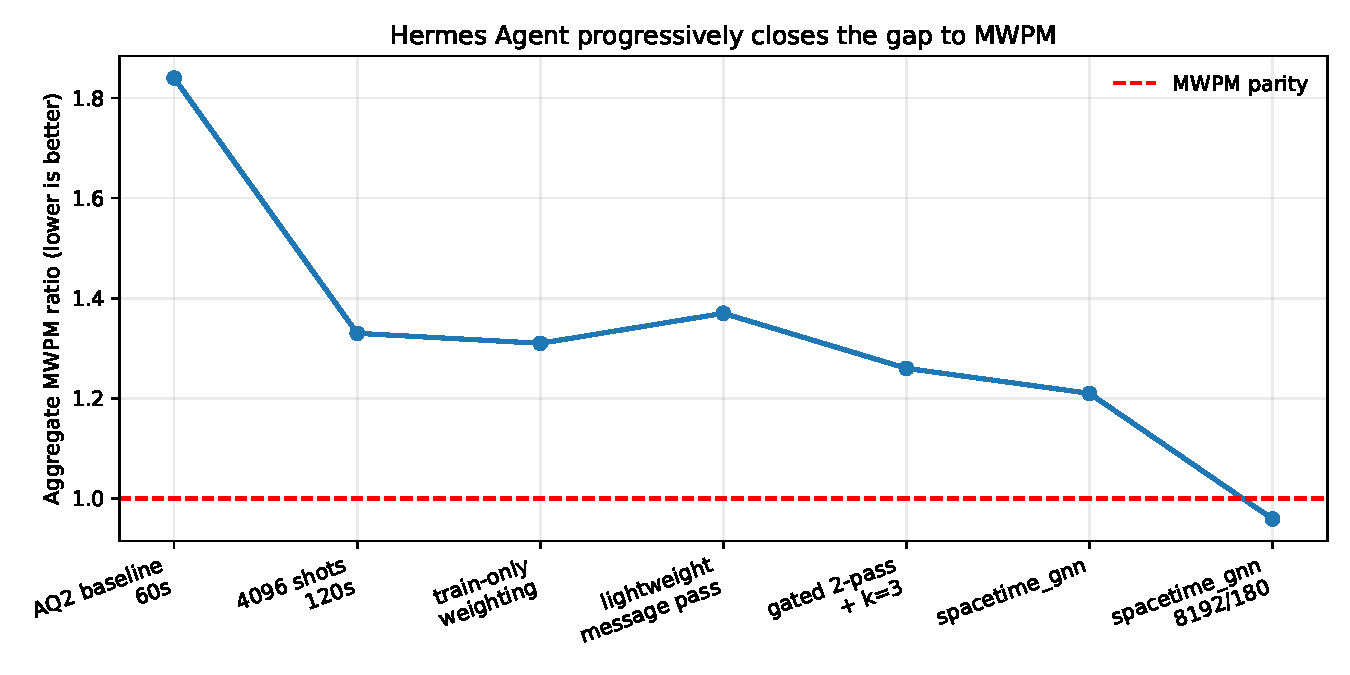
\includegraphics[width=\linewidth]{figures/milestone_progress.pdf}
    \caption{Aggregate MWPM ratio over major milestones in the project. The largest improvements came from (i) more data and more time, (ii) graph priors, and finally (iii) a full space-time graph decoder. The dashed line marks MWPM parity.}
    \label{fig:progress}
\end{figure}

\section{Setting and benchmark policy}
The repository operates on deterministic local surface-code profiles with fixed train/validation caches and machine-readable training/evaluation artifacts. In the period covered by this paper, the work concentrated on the local-d3-v1 profile: distance 3, rounds 3, five physical error rates $p \in \{0.001, 0.003, 0.005, 0.007, 0.01\}$, and one logical observable.

A central outcome of the research process was a benchmark-policy update. Early experiments used train4096/val256 for both selection and promotion. However, repeated overnight runs showed that val256 was often too noisy to distinguish neighboring hypotheses reliably. The project therefore adopted train8192/val1024 as the primary research and promotion benchmark, while train8192/val256 was retained as a secondary continuity check. This change was itself a scientific result of the effort: benchmark noise can dominate local-search decisions in small-scale decoder tuning.

The primary scalar objective throughout was the aggregate MWPM ratio,
\[
\text{MWPM ratio} = \frac{\text{aggregate learned-decoder LER}}{\text{aggregate MWPM LER}},
\]
where lower is better and values below $1.0$ indicate beating MWPM on aggregate.

\begin{figure}[H]
    \centering
    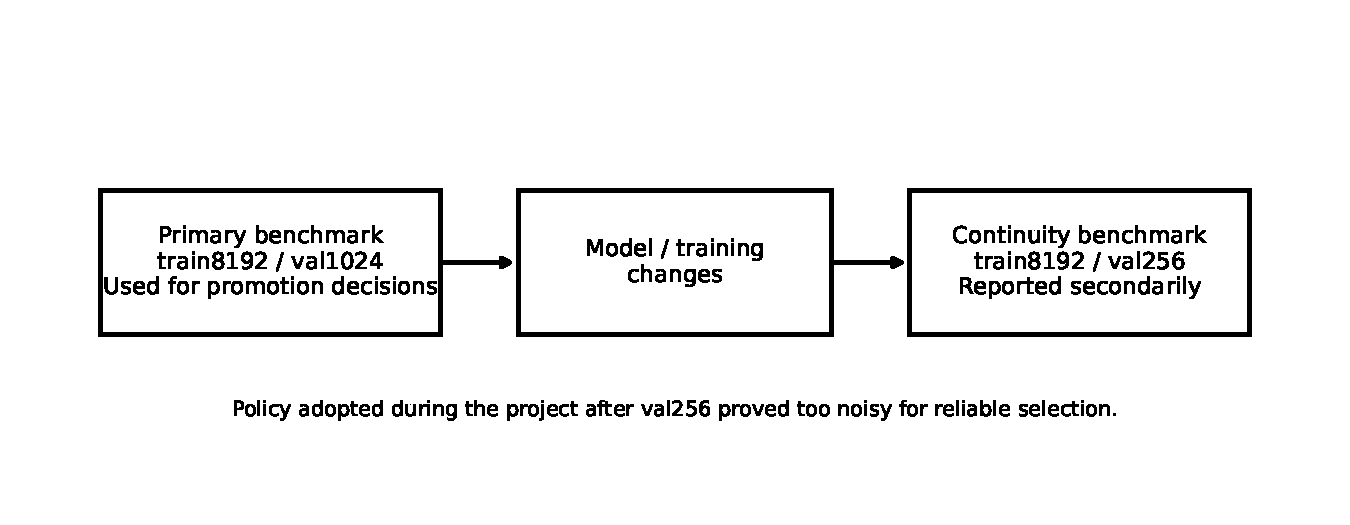
\includegraphics[width=0.95\linewidth]{figures/benchmark_policy.pdf}
    \caption{Benchmark policy adopted during the project. The larger validation benchmark became the primary decision rule, while the smaller validation benchmark was retained as a continuity check.}
    \label{fig:policy}
\end{figure}

\section{From AQ2 to graph-native decoding}
\subsection{Baseline family}
The initial model family used a stronger minimal AQ2-style decoder: detector-aware token embeddings, gated recurrence across time, and a per-bucket spatial transformer. Within this family, the agent found several robust lessons: Lion plus warmup-cosine scheduling was already well tuned; increasing train shots from 1024 to 4096 and extending the budget from 60s to 120s delivered the largest early gain; and replacing validation-driven slice weighting with train-only $p$-weighted sampling improved both methodology and performance. These changes moved the aggregate MWPM ratio from roughly $1.84$ down to roughly $1.31$, but repeated sweeps showed that plain width/depth/learning-rate tuning within the AQ2 family had diminishing returns.

\subsection{Lightweight graph priors}
The next phase introduced local message passing in the final AQ2 block. The critical discovery was not merely that message passing helped, but how it had to be introduced: graph reasoning worked best late in the network; a mild second pass helped more than a heavy-handed stronger pass; and slightly widening the local neighborhood to $k=3$ produced the best version of this family. These graph-augmented AQ2 variants drove the primary-benchmark ratio to about $1.26$, but still did not reach parity.

\subsection{Fuller graph-neural redesign}
The decisive next step was to stop treating graph structure as an auxiliary refinement and make it the backbone. We introduced a new model, \texttt{spacetime\_gnn}, which operates directly over detector nodes with typed spatial and temporal graph propagation. Conceptually, this shift is closer to relational graph reasoning than to another AQ2-style refinement, following the intuition behind relation-aware graph networks~\citep{Schlichtkrull_2018}. The model retains the existing detector, coordinate, time, and physical-error embeddings, but replaces the late corrective message pass with stacked typed graph blocks and a graph-native readout. Figure~\ref{fig:architecture} sketches the resulting pipeline.

\begin{figure}[H]
    \centering
    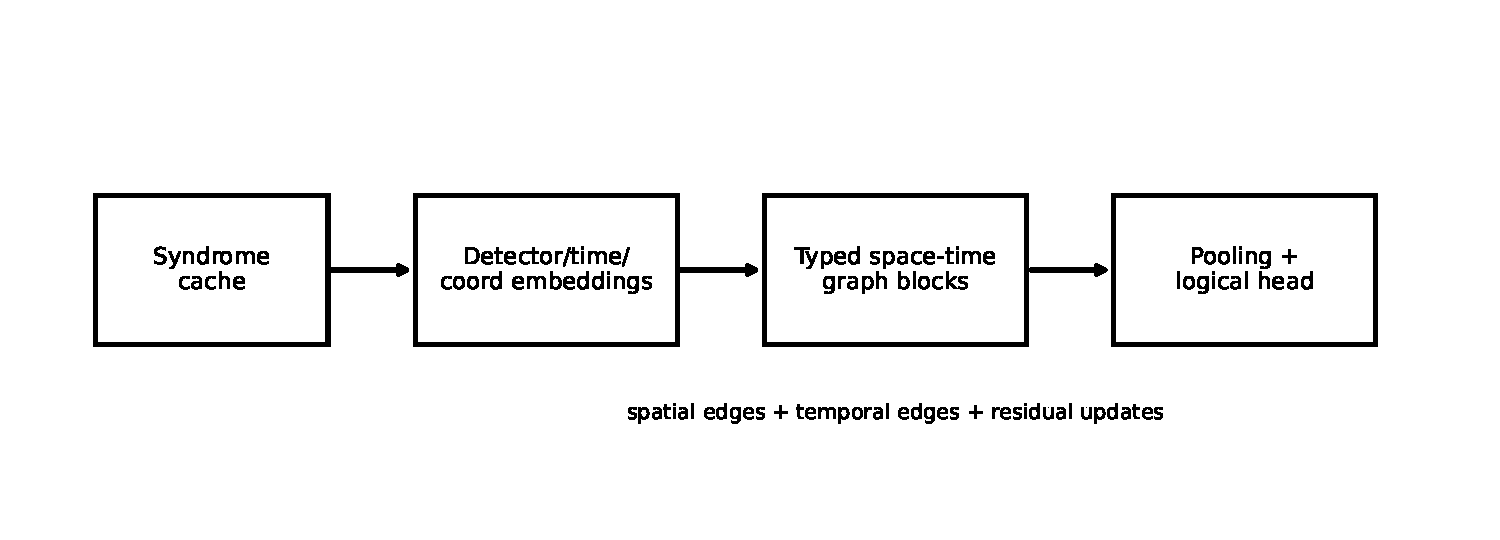
\includegraphics[width=\linewidth]{figures/architecture_overview.pdf}
    \caption{Overview of the promoted graph-native decoder family. Syndrome caches are embedded into detector/time/coordinate features, processed by typed space-time graph blocks, then pooled for logical prediction. The final promoted regime uses \texttt{spacetime\_gnn} with six graph blocks and wider feedforward updates.}
    \label{fig:architecture}
\end{figure}

The best promoted regime used \texttt{spacetime\_gnn} with six graph blocks, feedforward multiplier 6, 8192 train shots, and a 180-second budget. This final combination turned out to matter jointly: the richer graph-native model only paid off once it was given enough data and time.

\section{Experimental trajectory}
The entire effort can be summarized as a sequence of progressively stronger inductive biases. Table~\ref{tab:timeline} gives the compact changelog, while Figure~\ref{fig:progress} visualizes the same trajectory.

\begin{table}[t]
    \centering
    \small
    \caption{Compact milestone timeline for the decoder-improvement effort. Ratios are aggregate MWPM ratios on the contemporaneous benchmark used to judge that stage.}
    \label{tab:timeline}
    \begin{tabular}{p{0.26\linewidth}p{0.50\linewidth}r}
        \toprule
        Stage & Main change & Ratio \\
        \midrule
        AQ2 baseline & Lion + warmup-cosine AQ2 baseline & $\sim 1.84$ \\
        More data/time & 4096 train shots plus 120s budget & $\sim 1.33$ \\
        Train-only weighting & Train-only $p$-weighted sampling & $\sim 1.31$ \\
        First graph prior & Final-block message passing & $\sim 1.37$ \\
        Mild graph refinement & Gated second pass plus $k=3$ & $\sim 1.26$ \\
        Fuller graph redesign & \texttt{spacetime\_gnn} introduced & $\sim 1.21$ \\
        Final promoted regime & \texttt{spacetime\_gnn}, 6 blocks, FF$\times$6, 8192/180 & $\mathbf{0.959}$ \\
        \bottomrule
    \end{tabular}
\end{table}

\section{Related work}
This paper sits at the intersection of learned quantum-error-correction decoding, graph-based neural reasoning, and autonomous ML research workflows. On the decoding side, AlphaQubit demonstrates that learned decoders can achieve high decoding accuracy on quantum-processor data~\citep{Bausch_2024}. Our work differs in setting and intent: rather than proposing a single decoder from scratch, we document an autonomous iterative search process inside a local harness and show how graph-native redesign was necessary to cross the MWPM threshold on the primary repository benchmark.

On the systems side, Stim~\citep{Gidney_2021} provides the fast stabilizer-circuit simulation infrastructure that makes this style of repeated local experimentation practical. On the modeling side, our final transition from AQ2-style sequence modeling to a typed space-time graph decoder is conceptually closer to relation-aware graph learning~\citep{Schlichtkrull_2018} than to further transformer-style refinement. Finally, the surface-code framing follows the standard large-scale fault-tolerance perspective of~\citet{Fowler_2012}.

\section{Final results}
The final promoted regime achieved repeated aggregate MWPM ratio $0.959$ on the primary benchmark (train8192/val1024). Across the three repeated seeds, the results were 0.9420, 0.9565, and 0.9783. The continuity benchmark remained slightly above parity on average (mean ratio $\approx 1.054$), but the primary benchmark, which the project ultimately adopted for research and promotion decisions, was below MWPM on repeated evidence.

\begin{table}[t]
    \centering
    \caption{Final promoted regime on the two benchmark suites.}
    \label{tab:finalresults}
    \begin{tabular}{lccc}
        \toprule
        Benchmark & Seed 1 & Seed 2 & Seed 3 \\
        \midrule
        train8192 / val1024 & 0.9420 & 0.9565 & 0.9783 \\
        train8192 / val256 & 1.0000 & 1.0968 & 1.0645 \\
        \bottomrule
    \end{tabular}
\end{table}

Figure~\ref{fig:slices} shows the final per-slice MWPM ratios for both benchmarks. The primary benchmark confirms that the final regime substantially reduced all slice gaps, including the previously difficult mid-range slices.

\begin{figure}[H]
    \centering
    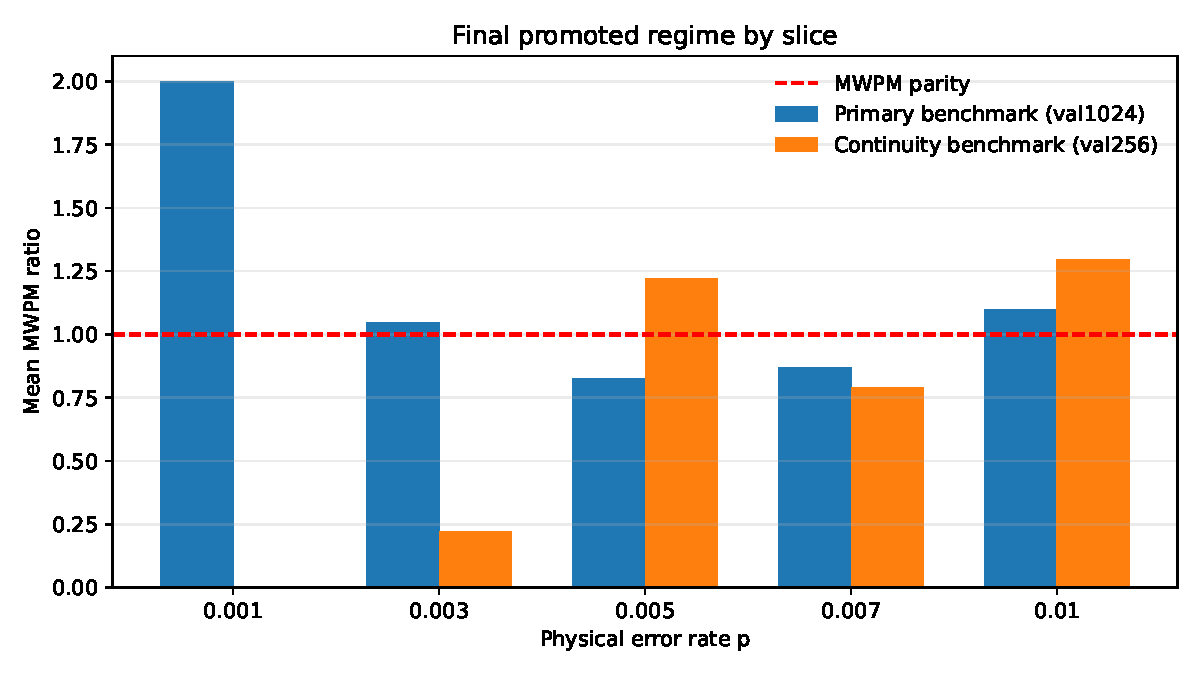
\includegraphics[width=\linewidth]{figures/final_slice_ratios.pdf}
    \caption{Per-slice MWPM ratios for the final promoted regime. The val1024 benchmark is primary; val256 is retained as a continuity check. The dashed line marks MWPM parity.}
    \label{fig:slices}
\end{figure}

\section{Why the final regime worked}
The retrospective across all runs supports three main conclusions. First, data and time were necessary but not sufficient: increasing train shots and training budget produced the largest early gain, but after that point the AQ2 family plateaued. Second, graph structure mattered more than generic capacity: plain width/depth increases in the AQ2 family often failed or produced noisy results, whereas graph-native structure unlocked further scaling. Third, the decisive shift was making graph reasoning primary rather than auxiliary. The breakthrough did not come from ever-stronger local corrections to AQ2; it came when the graph model became the actual backbone.

\section{Agent-driven research lessons}
This effort also functions as a systems case study in autonomous ML research. Repository contracts mattered because training, evaluation, and promotion artifacts were explicit. Benchmark policy mattered because moving from val256-led decisions to val1024-led decisions changed which hypotheses were worth pursuing. Open-ended agent loops benefited from a clear stopping rule: the loop stopped only when either the objective was reached or the remaining barrier clearly required a new project phase rather than more local search.

\section{Limitations}
This paper is a case study of one repository, one code family, and one local surface-code benchmark. It does not establish that autonomous agents can reliably speedrun arbitrary ML research programs, nor that the final promoted regime would transfer to larger distances, different noise models, or hardware datasets without further work. The benchmark policy changed during the project, and while that change was itself evidence-driven, it complicates strict historical apples-to-apples comparison across all stages. Finally, some of the conclusions are specific to the local-harness setting: a larger-scale research program would likely require additional statistical rigor, external validation, and compute accounting.

\section{Conclusion}
We set out to see how far an autonomous agent could push a local quantum-error-correction decoder before the problem ceased to be about tuning and became about architecture. Starting from an AQ2-style baseline far above MWPM, the system iteratively improved the decoder through more data, better training allocation, lightweight graph priors, and eventually a fuller space-time graph neural decoder. The final promoted regime beat MWPM on repeated evidence on the primary benchmark, with aggregate MWPM ratio $0.959$. The main scientific lesson is that graph-native inductive bias, not just more compute or more tuning, was the key to crossing the threshold. The main systems lesson is that open-ended agent research can be productive when the repository exposes crisp contracts, reproducible artifacts, and explicit promotion rules.

\FloatBarrier
\bibliographystyle{plainnat}
\bibliography{references}

\FloatBarrier
\appendix
\section{Architecture progression across model families}
This appendix provides more detailed diagrams for the main model families explored during the project. The goal is to make the architectural transitions explicit: from AQ2-style sequence modeling, to AQ2 augmented with local graph priors, and finally to a graph-native space-time decoder.

\begin{figure}[t]
    \centering
    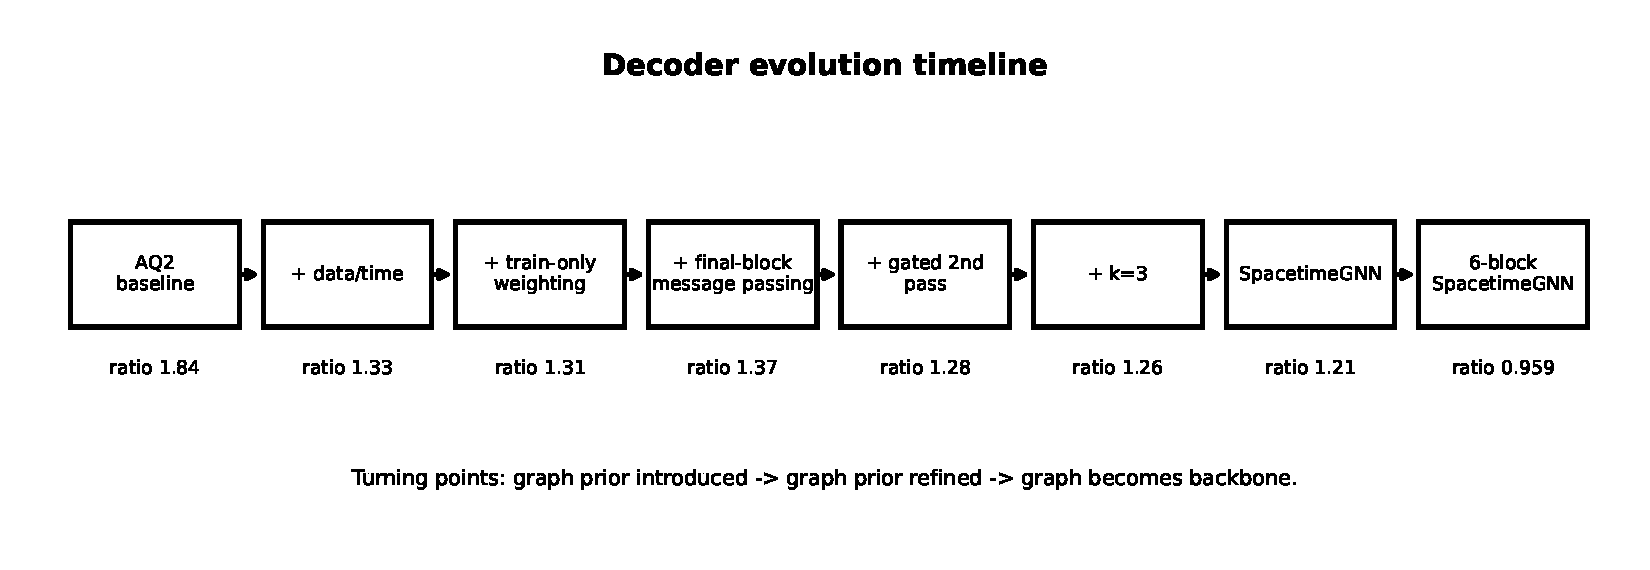
\includegraphics[width=\linewidth]{figures/appendix_evolution_timeline.pdf}
    \caption{High-level evolution timeline of the decoder families explored during the project.}
    \label{fig:appendix-evolution}
\end{figure}

\begin{figure}[t]
    \centering
    \begin{subfigure}{\linewidth}
        \centering
        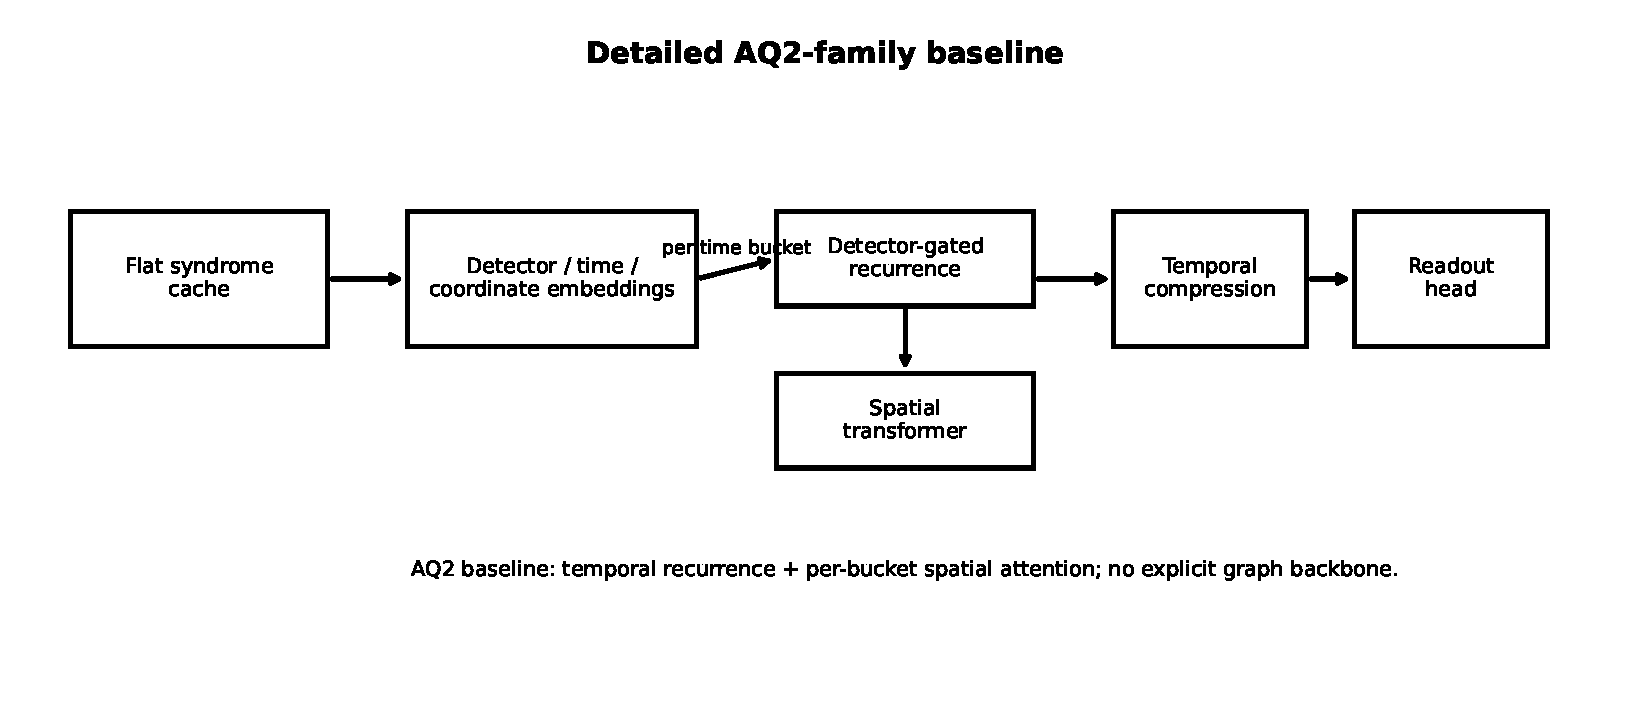
\includegraphics[width=\linewidth]{figures/appendix_detailed_aq2.pdf}
        \caption{Detailed AQ2 baseline architecture. Temporal recurrence and per-bucket spatial attention are the primary computation, with no explicit graph backbone.}
        \label{fig:appendix-detailed-aq2}
    \end{subfigure}

    \vspace{1em}

    \begin{subfigure}{\linewidth}
        \centering
        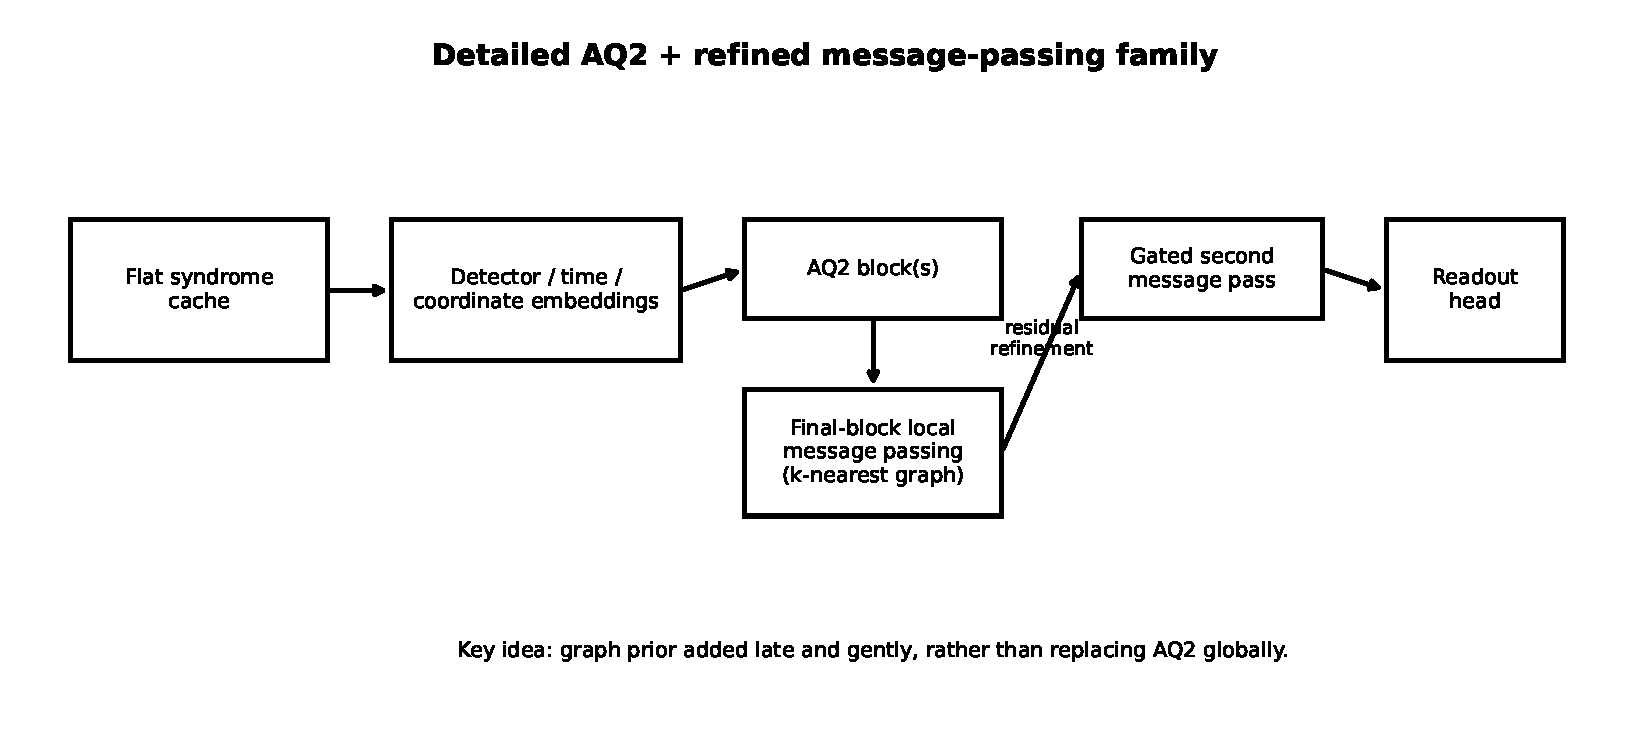
\includegraphics[width=\linewidth]{figures/appendix_detailed_aq2_mp.pdf}
        \caption{Detailed AQ2 + message-passing family. Local graph structure enters as a late correction in the final block, first through one message-passing pass and later through a mild gated second pass with a wider neighborhood.}
        \label{fig:appendix-detailed-aq2-mp}
    \end{subfigure}

    \caption{Detailed AQ2-family architecture progression.}
    \label{fig:appendix-detailed-aq2-family}
\end{figure}

\begin{figure}[t]
    \centering
    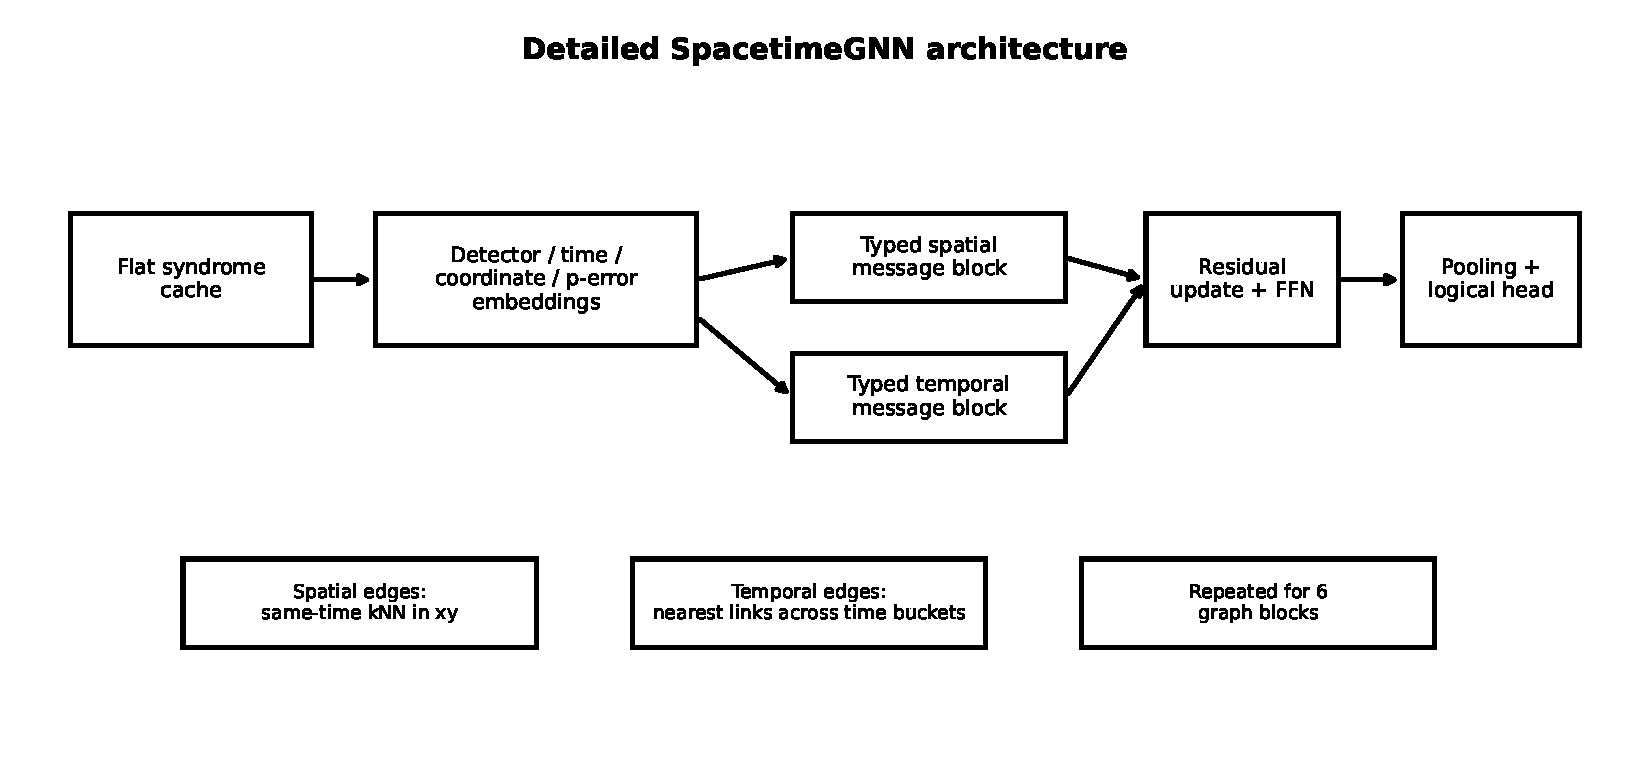
\includegraphics[width=\linewidth]{figures/appendix_detailed_spacetime_gnn.pdf}
    \caption{Detailed SpacetimeGNN architecture. Typed spatial and temporal graph propagation replace the late corrective graph prior with graph reasoning as the backbone.}
    \label{fig:appendix-detailed-spacetime-gnn}
\end{figure}

\FloatBarrier

\end{document}
